\documentclass{standalone}
\usepackage{standalone}

\begin{document}

\section{Character Recognition}
The character recognition is the final and most crucial part of the automated system. We decided to go with a straight-forward approach to implement a Multi-Layer Perceptron model to recognize characters. An MLP or Multi-Layer Perceptron is a Neural Network model that has only three layers. The input layer, one hidden layer and one output layer.

\subsection{Feature Extraction}
We have extracted 27 most basic features that shall help us to identify a character. We For each segmented characters we extracted same amount of features and passed it to the input of neural network for classification. Our selecting of feature effectively reduced the number of computations and made the system more efficient. We shall describe our approach to extract features here in brief.
\subsubsection{Feature 1 and 2}
There is a function in {\it numpy} library called {\it count\_nonzero} that counts the non-black pixels of the image. We used it to count the total non-black pixels of the initial image. This is our second feature.
\begin{lstlisting}[language=Python]
feature[1] = width * height
total_pixels = numpy.count_nonzero(img)
feature[2] = total_pixels
\end{lstlisting}

\subsubsection{Feature 3 and 4}
We divided the image into two parts horizontally (Figure \ref{fig:FeatureHor}). Our 3rd feature is the ratio between non-black pixels in the upper part and total pixels, and 4th feature considers total non-black pixels in lower part.
\begin{lstlisting}[language=Python]
center_x = width // 2
center_y = height // 2
up_pixels = numpy.count_nonzero(img[:center_x, :])
feature[3] = up_pixels / total_pixels
down_pixels = numpy.count_nonzero(img[center_x:, :])
feature[4] = down_pixels / total_pixels
\end{lstlisting}

\begin{figure}
\centering

\includegraphics{img/feature/hor}
\caption{Dividing image into upper and lower areas}
\label{fig:FeatureHor}
\end{figure}

\subsubsection{Feature 5 and 6}
Similarly we divided the image vertically (Figure \ref{fig:FeatureVer}), and extracted our features from left and right side respectively.
\begin{lstlisting}[language=Python]
left_pixels = numpy.count_nonzero(img[:, :center_y])
feature[5] = left_pixels / total_pixels
right_pixels = numpy.count_nonzero(img[:, center_y:])
feature[6] = right_pixels / total_pixels
\end{lstlisting}

\begin{figure}
\centering

\includegraphics{./img/feature/ver}
\caption{Dividing image into left and right areas}
\label{fig:FeatureVer}
\end{figure}


\subsubsection{Feature 7 to 10}
Now we divide the image into four parts (Figure \ref{fig:FeatureFours}). And calculate the non-black pixels ratio on each parts.
\begin{lstlisting}[language=Python]
up_left_pixels = numpy.count_nonzero(img[:center_x, :center_y])
feature[7] = up_left_pixels / total_pixels
up_right_pixels = numpy.count_nonzero(img[:center_x, center_y:])
feature[9] = up_right_pixels / total_pixels
bottom_left_pixels = numpy.count_nonzero(img[center_x:, :center_y])
feature[8] = bottom_left_pixels / total_pixels
bottom_right_pixels = numpy.count_nonzero(img[center_x:, center_y:])
feature[10] = bottom_right_pixels / total_pixels
\end{lstlisting}

\begin{figure}
\centering

\includegraphics{./img/feature/fours}
\caption{Dividing image into 4 areas}
\label{fig:FeatureFours}
\end{figure}

\subsubsection{Feature 11 to 26}
Next we divide the image into eight parts (Figure \ref{fig:FeatureEights}). And similarly calculate the feature for each parts.
\begin{lstlisting}[language=Python]
qx = height // 4
qy = width // 4
four = range(0, 4)
for i in four:
    for j in four:
        x1 = i * qx
        x2 = (i + 1) * qx
        y1 = j * qy
        y2 = (j + 1) * qy

        pixels = np.count_nonzero(img[x1:x2, y1:y2])
        feature[11 + 4*i + j] = 100 * pixels / total_pixels
    # end if
# end if
\end{lstlisting}

\begin{figure}
\centering

\includegraphics{./img/feature/eights}
\caption{Dividing image into 16 parts}
\label{fig:FeatureEights}
\end{figure}

\subsubsection{Feature 27}
The final feature is calculated using the average of the euclidean distance between all the black pixels from central point (Figure \ref{fig:FeatureDist}).
\begin{equation}
feature[27] = \dfrac{1}{total\_pixels} \times \sum_{y}{\sum_{x}{ \sqrt{(x-center\_x)^2 \times (y-center\_y)^2} }}
\end{equation}


\begin{figure}
\centering
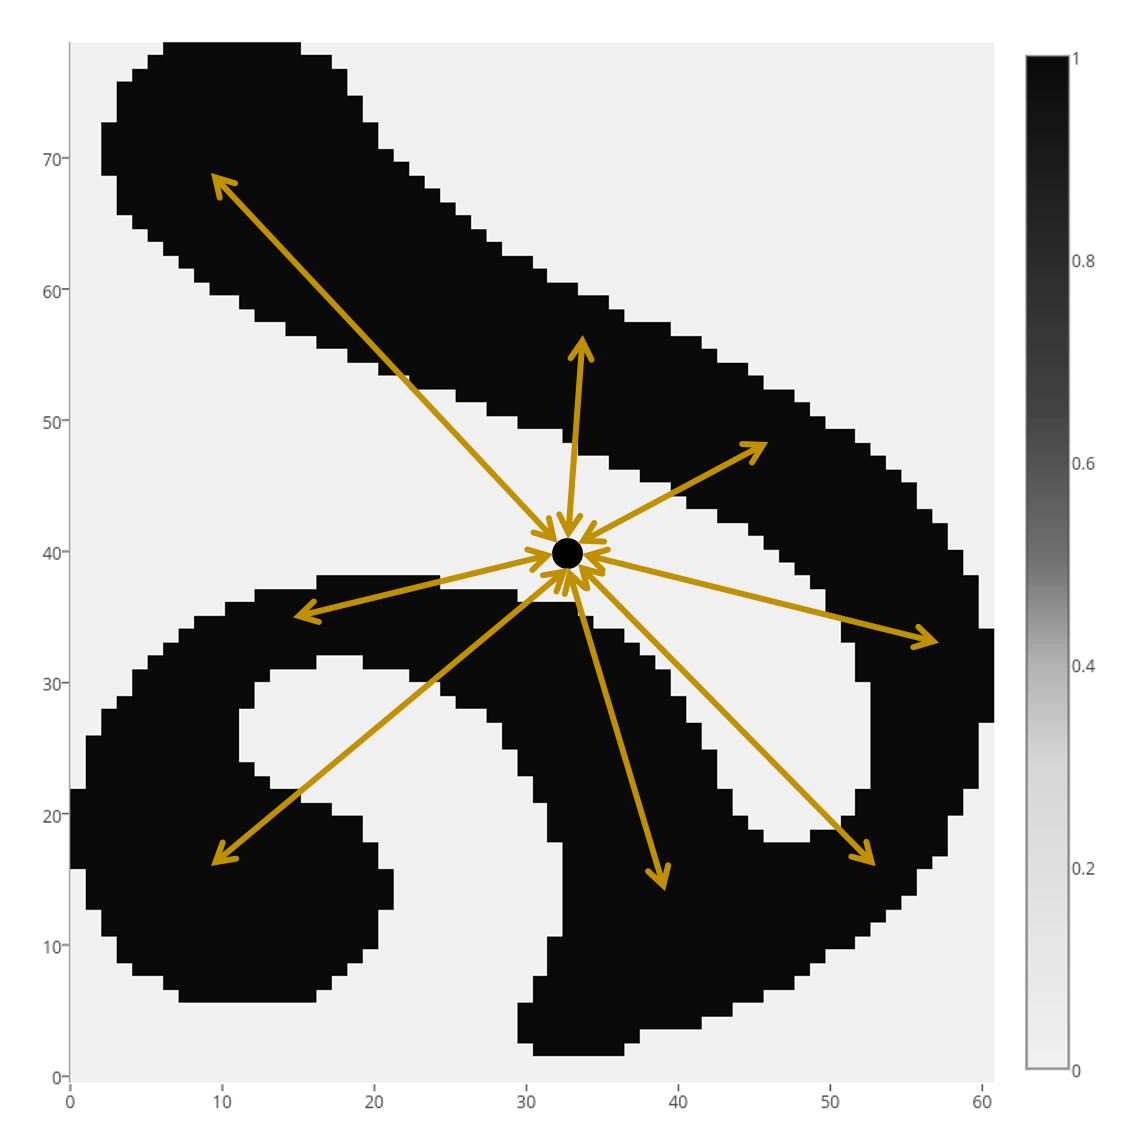
\includegraphics[width=0.8\linewidth]{./img/feature/dist}
\caption{Distances of non-black pixels from center.}
\label{fig:FeatureDist}
\end{figure}








\subsection{Neural Network Design}
A three layer feed forward supervised network is designed. The input layers has 25 neuron, taking the 25 extracted features from the previous step. 


\subsection{Training Process}
Due to the diversity and complexity of Bangla letters this stage is very challenging. But the Tesseract OCR needs to be trained properly before being able to recognize the license plate characters.

\subsection{Collecting training data}
The training database should have several images for each set of license plate characters, with the combination of various fonts and positions of the characters. In detected license plate, it is well possible for the characters to be rotated or skewed in more than 15 degrees. We used original character segments from the previous steps and as well as many auto-generated characters with different fonts, angles, and rotation. 

After the training database is collected, we had to convert all of the images into same format. We used ImageMagick to convert the training document to {\it tif} format. After formatting all the documents, we named had to name them properly. 

\subsection{Training the Tesseract OCR}
We run the python module for Tesseract OCR over the training dataset once it is ready. 




\end{document}